
\section{Introduction}
\label{sec:intro}

The area of artificial intelligence has achieved substantial advancements in recent years, notably through the development of Large Language Models(LLMs) \cite{achiam2023gpt,meta2022human,ouyang2022training} . LLM-as-Agent is one of the popular applications \citep{yao2022react,zhu2023ghost,zhao2024expel}, with particular focus on multi-agent communication technology receiving widespread attention \citep{qian2023communicative,li2023camel,wang2023avalon}, showcasing fascinating phenomena and emergent cooperative behaviors. Meanwhile, how to apply LLM agents to social deception games, such as Werewolf \citep{xu2023exploring,wu2024enhance}, Avalon \citep{wang2023avalon,light2023avalonbench}, and One Night Ultimate Werewolf \citep{jin2024learning}, has also become a popular research direction. However, these study and frameworks often focus on the statistical outcomes, like the accuracy of prediction or the win rate, while overlooking another significant characteristic of LLMs-their inherent randomness, which can provide enrichment to the game content.

The scope of human behavior is broad and complicated \citep{riedl2012interactive,yannakakis2012game}.Thus, we should investigate the potential of LLM agents in generating diversity and richness as simulators of human behavior. It is observed that the search results generated by LLMs exhibit a certain degree of randomness \citep{yadkori2024believe,hendrycks2020measuring}, which is a challenge for accuracy-seeking strategies but a treasure for creators aiming for aboundance and richness. For instance, Generative Agent \citep{park2023generative} implemented a sandbox simulation framework that allows LLM agents to freely develop daily plans, showcasing the potential for AI to autonomously create lifelike scenarios. Other researchers have discovered that LLMs can be leveraged to introduce deceptive elements into conversations within social games \citep{wang2023avalon}. Attempts at building a dual-system modeling based on a psychological theory \citep{wu2024enhance} have also imbued LLM agents with a degree of anthropomorphism. In fact, LLM-as-Agent, as a form of AI simulating human behavior, has yet to fully explore the depth and breadth of its capabilities. We still require the integration of psychological methodologies and the incorporation of simulations of real human decision-making to construct agents that better reflect the broad spectrum of human behavioral space.

\begin{figure*}[ht]
  \centering
  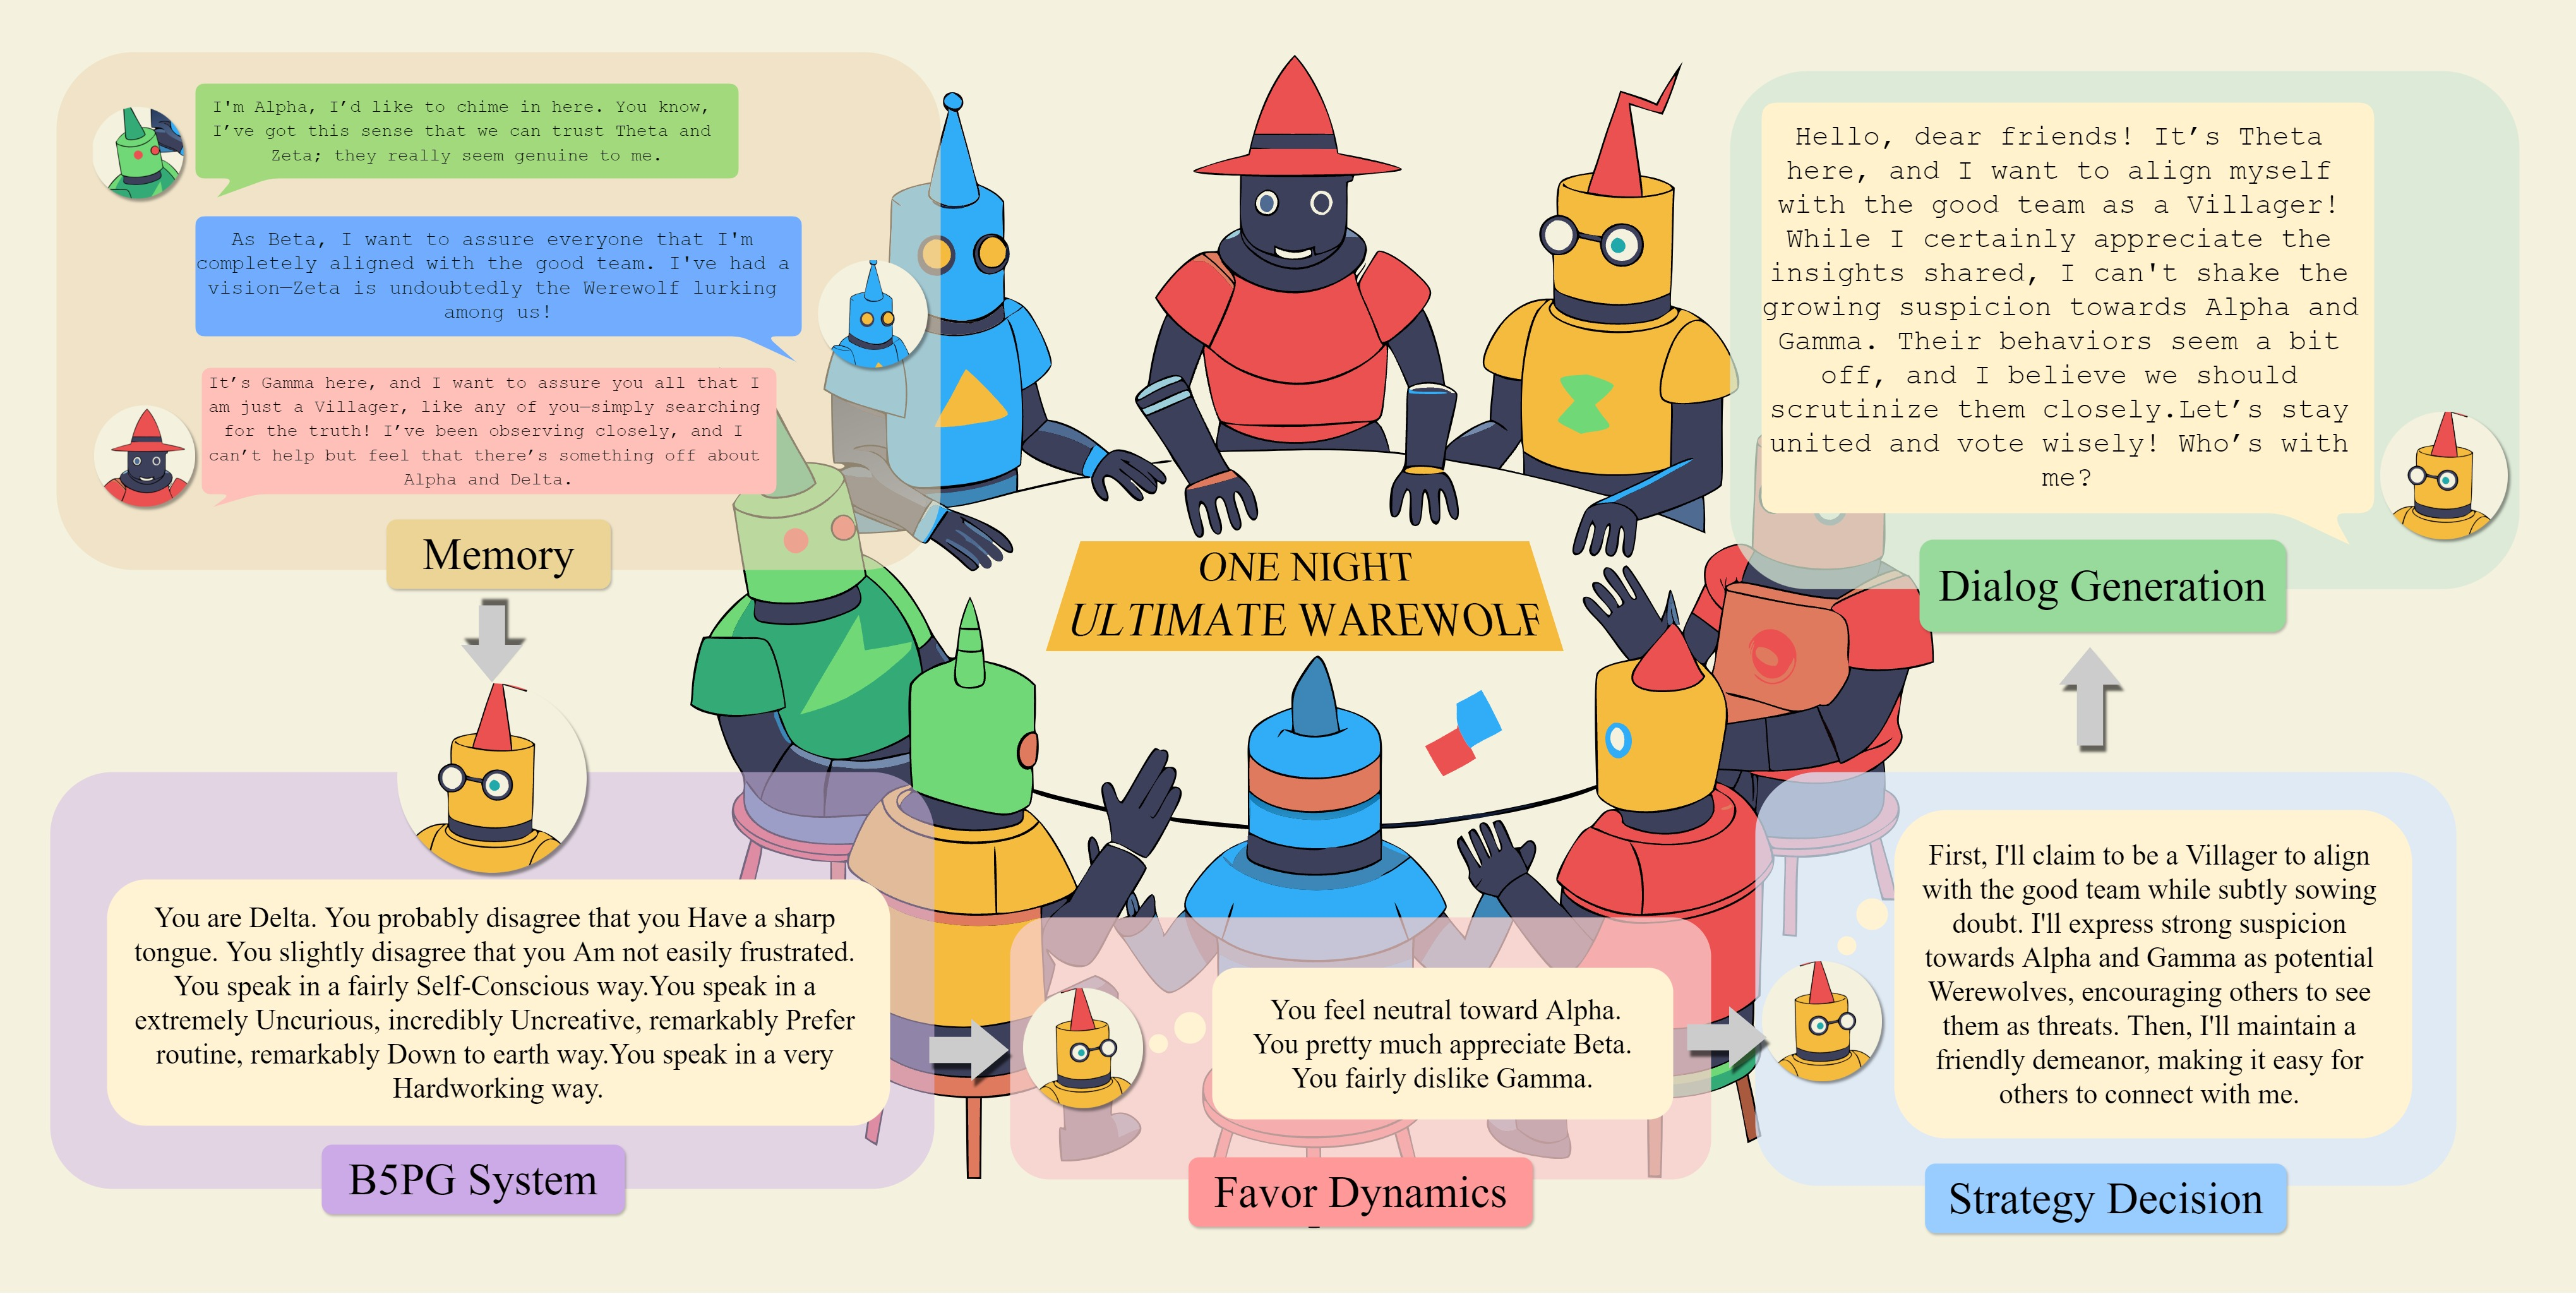
\includegraphics[width=0.99\textwidth]{img/dialog.jpg}
  \caption{ \textbf{The introduction of the framework of Our Humanized Agents}  }
\label{fig:dialog}
    \vspace{-1em}
\end{figure*}

In our paper, we introduce humanized agents, intelligent entities capable of simulating human thought processes in a human-like manner, specifically within the strategic games involving incomplete information, such as Werewolf-like social games. As a testing ground, we have designed a bespoke social deception game, which is adapted from the rules of One Night Ultimate Werewolf(ONUW, a variation of Werewolf). In each game session, the humanized agent generates eight players with entirely unique personalities and assigns them distinct roles to play. Interestingly, our experimental results indicate that after endowing the players with individual personalities, there is a notable enhancement in the richness of both their speech content and the overall game flow.

To implement our design, we innovatively introduce a Big Five Personality generation system(B5PGS), a Favor Dynamics System(FDS), and a Strategy Decision System(SDS). Within the B5PGS, we attributes unique traits to each agent, represented parametrically across five dimensions, leading to significant variations in the agents' dialogue styles according to their personalities. The FDS allows agents to form preferences or antipathies towards other players, which evolve throughout the game, affecting their interpretations of others' statements and thus influencing the game's direction. With the introduction of SDS, inspired by the Chain of Thought(CoT) \citep{wei2022chain} and dual decision system \citep{wu2024enhance}, agents independently make decisions about the course of conversations, enabling them to better disguise their identities and engage in deception. Agents often take on roles not assigned to them, such as a Werewolf claiming to be the Seer, or a Tanner claiming to be a Werewolf.



Moreover, we creatively propose several evaluation methods for textual diversity. Since our research does not focus on the win-loss outcomes of each faction in the game, we cannot simplily analyze the win rates of each team. Therefore, we defined three approaches to quantify the diversity of output content: evaluating text distance; evaluating judgement variation; and assessing game content using large language models. Text distance is calculated by first embedding the dialogues of each agent in the game \citep{mikolov2013efficient} and then computing the distance between these vectors. This method quantitatively reflects the richness of language use within the game. Judgemen variation refers to the statistical analysis of voting counts in each round and examines the distribution of votes across different characters in various game sessions. A more even distribution indicates that the identities of each player are less clear (which leads to votes being cast for different roles), thereby increasing the uncertainty and enjoyment of the game. Evaluation using large language models \citep{shao2023character,wang2024incharacter} involves scoring the quality of dialogue content with these models. This approach enables the quantitative assessment of dimensions that are otherwise difficult to measure, such as interest, attraction, and surprise.

In sum, the main contributions of this paper lie in:

\begin{itemize} 
  \item {\bf Humanized agents}, capable of simulating individuals with different personality traits, and for language-based strategic games, able to continuously adjust the strategies dynamically based on feedback from other players.
  \item {\color{red}}Empirical studies on Werewolf demonstrate that our framework demonstrates the ability to learn from experiences without tuning the parameters of LLMs.
  \item Strategic behaviors such as trust, confrontation, camouflage, and leadership begin to emerge in our experiments, which can serve as a catalyst for further research on LLMs for communication games.
\end{itemize}